\newcommand\SLASH{\char`\\}

\section{Protocol Design}
\label{protocol_design}

\subsection{Protocol Overview}

\begin{figure}[!h]
    \begin{center} %should there even be more than one "client" bubble in this diagram?
        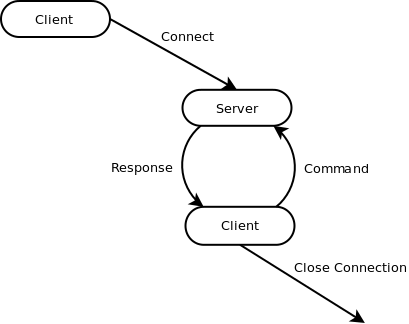
\includegraphics[scale=0.65]{Design/diagrams/protocol_high_level.png}
        \caption{The exchange of messages between a client and the server}
        \label{highLevelDia}
    \end{center}
\end{figure}

GIM uses a client-server architecture, where one computer (known as the server) acts as a central point to which other computers (the clients) connect. The clients do not communicate directly with each other. If a client wishes to send a message to another client it must first got through the server.
%protocol: capitalized or no?
A protocol is a set of rules that determine the format and transmission of data between computers. In GIM, the Protocol is responsible for enabling communication between the clients and the server in a reliable and consistent manner.  The syntax (the structure, or format) and semantics (the meaning) of the Protocol are discussed in the next section.

At the highest level of abstraction, the GIM Protocol works in a very simple manner.  A client connects to the sever and they exchange messages until the connection is closed, as shown in Figure ~\ref{highLevelDia}.

In practice there are several clients connected to the server at once, however as the clients do not directly interact with each other and do not need to know about each other, the entire system can be described as above.


\subsection{Syntax}

The GIM Protocol uses a simple, text based syntax. Each full command begins with a colon followed by a command name and its arguments. A second colon marks the end of the header and beginning of the data segment. A semi-colon marks the end of the data segment and the termination of the command. The basic structure of a full command is shown below:

\texttt{:<COMMAND\_NAME> <ARGUMENTS>: <DATA>;}

Commands names are predefined and \texttt{<COMMAND\_NAME>} can be any 1 of the following 19 values:

\texttt{
\begin{tabular}{ | p{3.3cm} |p{3.3cm}  |p{3.3cm} |p{3.3cm} | } 
    \hline
    AUTH & FRIENDREQUEST & MESSAGE & ROOM \\
    \hline
    BROADCAST & GET & OKAY & SERVERSTATUS \\
    \hline
    ERROR & INFO & PING & SET \\
    \hline
    FRIEND & KILL & PONG & UPDATE \\
    \hline
    FRIENDLIST & LOGOUT & QUIT & \\
    \hline
 \end{tabular}
}
 
\texttt{<ARGUMENTS>} is a set of zero or more predefined arguments which can be passed to the command in order to change its behaviour. Each command has its own set of arguments. Some commands require arguments (sometimes more than one) and some commands have no arguments. The protocol specification defines over 60 arguments, and a full listing for each command can be found in Appendix \ref{protocol_spec}.

Unlike the command and argument segments, the \texttt{<DATA>} segment does not have any predefined values and has a varying syntax across different commands.  For example, the \texttt{:ROOM:} command has \texttt{:JOIN:} and \texttt{:LEAVE:} arguments which are used to join or leave a chat. The majority of the data is likely to have been provided by the user at some point, and as such the data segment is considered to be ``unsafe.'' This data is encoded (see section \ref{encoding} for more information). A full specification for the data segment of each command can also be found in Appendix \ref{protocol_spec}.

For example, the following is an example of a command sent from the client to the server requesting the Nickname and Status of the users joe@example.com and bill@gmail.org:

\texttt{:GET NICKNAME STATUS: joe\SLASH U+0040example.com bill\SLASH U+0040mail.org;}

To which the server may reply:

\texttt{:INFO NICKNAME STATUS: joe\SLASH U+0040example.com\\
Jeo\\
ONLINE\\
bill\SLASH U+0040mail.org\\
Billy The Kid\\
AWAY;}

The data segments in the previous examples have been encoded as defined below in section \ref{encoding}.

\subsection{Roles and States}

The protocol defines two separate roles: The Client role and the Server role. Each role is only able to send a specific subset of commands and receive all of the commands sent by the opposite role (i.e. the server must understand all of the commands which the client is able to send and vice-versa). This means that both the client and server must implement all commands.

Having clearly defined roles is an integral part of the GIM Protocol. This allows the semantics of a command to generate a response. Both roles are able to send and receive commands, but the commands have different meanings depending on their source. 

For example, the \texttt{:AUTH:} command can be sent by both the client and the server. When sent by the server it is used to indicate the current state of the client (Either Logged-in or Unauthorized) but when sent by the client it indicates that a user wishes to login or register a new account. This means that the same command must be implemented differently depending on the role of the sender.

As mentioned above, the client role has 2 states: Logged-in and Unauthorized. When the client first establishes a connection it is placed in the unauthorized state. This means that it has access to an even smaller subset of commands, only those essential to logging-in or registering a new account. Once the client has successfully logged-in, it is granted access to the full set of client commands.


\subsection{Encoding, Limits and Restrictions}
\label{encoding}

Any non-letter or digit (anything not a-Z or 0-9) in the data segment of a command is encoded and replaced by \texttt{\SLASH U+} followed by a 4 digit number representing the UTF-16 code for the character. For example, the @ character in the previous example is encoded as \texttt{\SLASH U+0040}. The only exception to this rule is a character which is used to format or separate different chunks of data. In the GIM Protocol this is always either a single space (the equivalent of \texttt{\SLASH U+0020}) or a newline character (\texttt{\SLASH n}).

Display pictures, which are small images in JPEG format, cannot be transferred easily using the GIM Protocol without first being converted to a text based format. JPEG and any other binary data is encoded using BASE64 encoding which is widely used and fairly efficient in terms of bandwidth and processing time.

This makes the protocol very easy to parse as we can safely split the data segment into separate parts without worrying about how data from the user is formatted. This means we can guarantee that every occurrence of a white-space character in the data segment is safe to use for splitting the data.

Clients connected to the server are limited to sending 100 commands in a rolling 5 second window. Normal usage should result in a much lower rate (less than 5 per second) and anything more than than this most likely indicates a malfunctioning or malicious client. In the event a client exceeds this limit, the server closes the connection with the client.

The data segment of commands sent by the client is limited to 8192 characters in length. This includes data that has been encoded, so a single @ character encoded as \texttt{\SLASH U+0040} counts for 7 characters towards the limit. The only exception to this rule is the \texttt{:SET DISPLAY\_PIC:} command, which is used to set a users display picture. The limit for this command is 4x greater than that of a normal command (32,768 characters or around 24kb worth of JPEG data). The server has no such limits and can send commands of any length.

\subsection{Heart Beat}

In order to ensure that clients are working correctly and have not disconnected or crashed without closing the connection, the protocol specifies that a client should send at least 1 valid command every 15 seconds. This can be problematic if the client is sitting idle as the vast majority of commands have side effects which may be undesirable. In order to avoid this the protocol has the \texttt{:PING:} and \texttt{:PONG:} commands. The \texttt{:PING:} command can be sent by the client at any time to signal that it is still active, without any side-effects. The server will always respond with the \texttt{:PONG:} command, which got its name in an attempt to bring some humour into the protocol.

\subsection{Error Handling}

The protocol specifies an \texttt{:ERROR:} command which the server may send if it has received a command it cannot fulfill. Almost all of the commands which can be sent by the client, with the exception of the \texttt{:PING:} command, can generate an \texttt{:ERROR:}. The specific type of error is signified by the arguments of the command, for example, an attempt to login with incorrect details might yield \texttt{:ERROR LOGIN\_DETAILS\_INCORRECT:;}.

The \texttt{:ERROR:} command can be very cumbersome to use as there are a very large number of arguments (usually several for every different command) and it can be difficult to match an error to a command as there is no identification of the command which caused it. Possible changes to address these issues are discussed in section \ref{protocol_evol}.

\subsection{Client-Server Interaction}

Once a client has entered the logged-in state it is able to send any command at any time, and in any order. The server is also able to send unsolicited commands to the client such as invites, updates and messages. As such, both the client and server have to be able to operate in a stateless way, treating each command they receive separate to all other commands. It is quite possible, and reasonable, for a client to send several commands to the server before it receives a response to the first. This eliminates the need to wait between some commands and allows for much more efficient client-server communication.

\newpage
\begin{landscape}
    \begin{figure}[!h]
        \begin{center}
            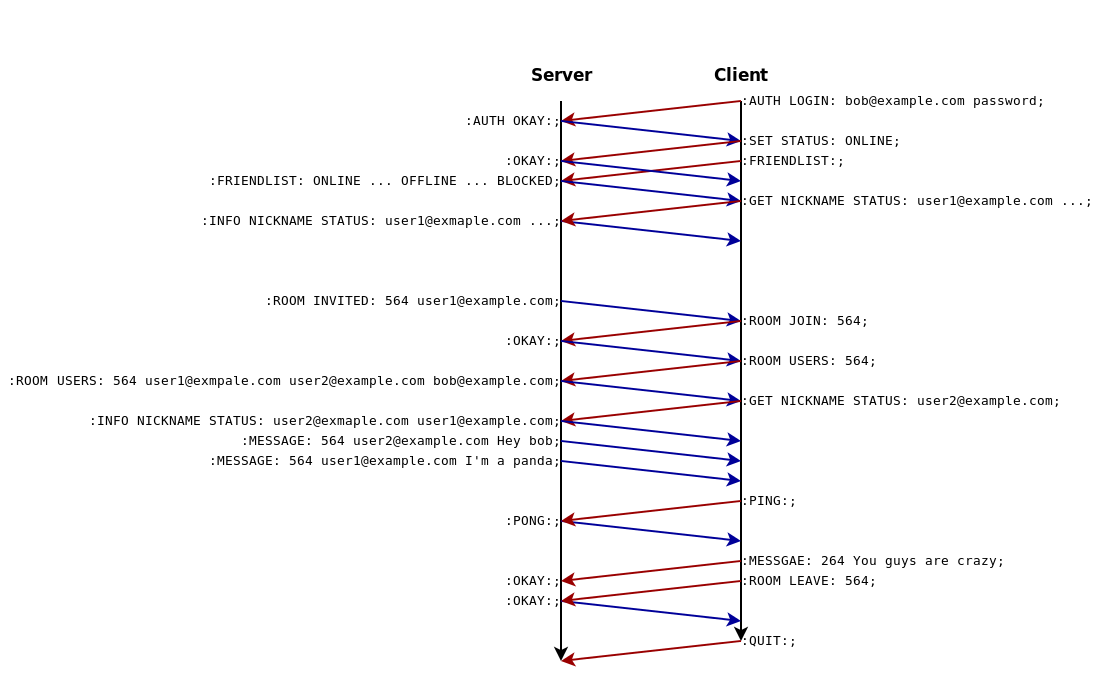
\includegraphics[scale=0.60]{Design/diagrams/protocol_interaction.png}
            \caption{Interaction diagram showing the exchange of messages between the client and server. Please note that the commands have NOT been encoded in order to improve readability. Some messages have been shortened and unimportant parts replaced by ...}
            \label{interactionDia}
        \end{center}
    \end{figure}
\end{landscape}

Figure \ref{interactionDia} shows typical usage of the GIM protocol. The following is a detailed description of the diagram.
\begin{enumerate}
\item{A client connects, attempts to log in using the \texttt{:AUTH LOGIN:} command, and waits for a reply.}
\item{The server responds \texttt{:AUTH OKAY:} signifying that the information was correct and the user has been logged in.}
\item{The client sets the user's status to ONLINE and immediately requests the user's friendlist from the server, without waiting for a response to the \texttt{:SET STATUS:} command.}
\item{The client receives the user's friendlist from the server and issues a \texttt{:GET:} command requesting the nickname and status of everyone in the friendlist.}
\item{The server receives the \texttt{:GET:} commands and responds with an \texttt{:INFO:} command containing the requested data.}
\item{Several seconds later the user is invited to a room and attempts to join it.}
\item{The server responds to the request to join the room with \texttt{:OKAY:} and the client requests a list of users in the room.}
\item{The server sends the client a list of users in the room, including themselves.}
\item{Two messages are sent to the room by other users and the server sends them to the client.}
\item{The client notices that it has not sent any commands for few seconds and sends a \texttt{:PING:} command to signal that it is still active.}
\item{The user sends a message to the room then leaves it.}
\item{The client sends the \texttt{:QUIT:} command to the server and closes the connection. The server logs the user out and closes the connection.}
\end{enumerate}

\subsection{Protocol Evolution}
\label{protocol_evol}

The GIM Protocol has undergone several significant changes since its first draft, such as the addition of different types of rooms and the removal of commas as separators to simplify the data segment. The most notable of these however was a move toward a smaller number of commands. This was done by merging similar commands together and allowing their behaviour to be modified by arguments. The number of commands was cut from 30 to 19, and resulted in a much easier to understand and more consistent protocol. Although this hid some of the complexity at a high level, it means that many of the commands are more complex. Overall this trade-off has been worthwhile and has made the protocol easier to use, at the cost of being slightly harder to implement.

A prime example of this is the \texttt{:FRIEND:} command. What was originally 6 separate commands to manage a user's friend list (adding, deleting, blocking, accepting friend requests, etc.) became a single command with several possible arguments. This grouped the related functionality of each command together. While the single command is more complex, it is still easier to use and remember than 6 separate commands.

There are still some commands which could arguably benefit from being merged. For example, it would make sense for the \texttt{:LOGOUT:} command to be part of the \texttt{:AUTH:} command which allows clients to login and register; all of these actions are conceptually similar. However, the \texttt{:LOGOUT:} command is not available unless the user is in the logged-in state, so one could argue that it should not be part of the \texttt{:AUTH:} command. The decision to keep them separate was made purely on personal preference as there were no clear advantages for either choice. 

During the implementation of GIM there were several modifications made to the format of the data segment for some commands. These were brought on by a desire to keep the protocol consistent across all commands. There was often a sense of confusion about how the data segment for each command was split into sections as each command had a different format; some used newlines, some used commas, and some used spaces as separators. In the end we chose to use spaces as separators in all commands except the \texttt{:INFO:} command where newlines made more sense. 

(Something about errors and how to improve the current situation)

(Could have made encoding more efficient by not using \texttt{\char`\\ U+}, use something shorter.)

The protocol has changed considerably since its first draft and has undergone substantial improvements in terms of ease of use, simplicity, and consistency. Although there are still some minor tweaks which could be made to further the improvement the protocol, it is currently in a stable and usable state. Future extensions to the protocol might include the addition of support for other features such as file transfers and VoIP.
